
\clearpage\subsection*{3−1 CGIについて勉強しよう}
\refstepcounter{PagePtr}\label{P:CGI}
ここではCGIについて勉強しよう。第1回で作成したwebページはいわば静的なページです。静的なページとは、常に同じ画面を表示するページのことです。ですが、CGI(Common
Gateway
Interface)を用いることによって動きのあるページ、動的なページを作成することができます。動的なページとは表示させるたびに違う画面を表示することができるページのことです。アクセスカウンターはたまにwebページについていることがあります。アクセスカウンタというのは、そのwebページに今までどれぐらいの人がアクセス(接続)したのかを表示させるものです。webページにアクセスするたびにアクセスカウンタの数は\ruby{増}{ふ}えていき、毎回同じ数字にはなりません。これはアクセスするというアクションによってページに変化を起こしているのです。さらにCGIを用いることによって以下の機能を作成することができます。


\bigskip


\centering
\begin{minipage}{\textwidth}
          \begin{minipage}{0.45\textwidth}
	   \textbf{・アクセスカウンター}\\
	   \centering
            {\upshape
              \centering
              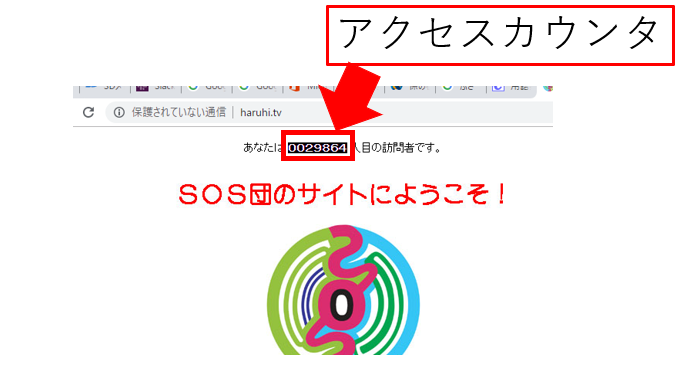
\includegraphics[width=0.8\linewidth]{ome7-img046.png}}
          \end{minipage}
          \begin{minipage}{0.45\textwidth}
	   \textbf{・アンケートフォーム}\\
	   \centering
            {\upshape
              \centering
              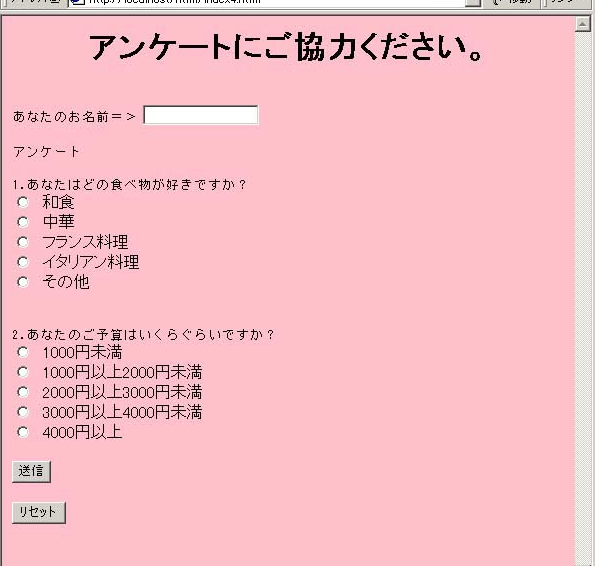
\includegraphics[width=0.8\linewidth]{ome7-img047.png}}
            \end{minipage}
\end{minipage}
\flushleft


\bigskip

{\bfseries

	・\ruby{掲示板}{けいじばん}}



\centering
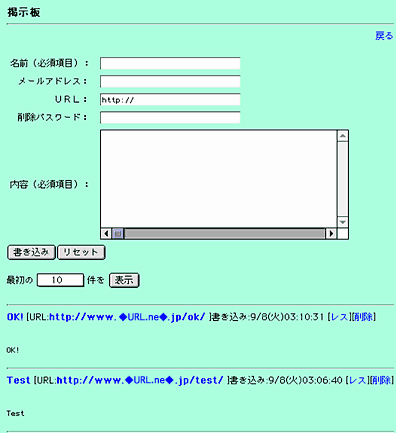
\includegraphics[width=4.431cm]{ome7-img048.png}
\flushleft





\bigskip

みんなが作ったwebページやほかの静的なページはどのようなやり取りで表示させているか見ていきましょう。次の図を見てください。

\bigskip

\clearpage


\centering
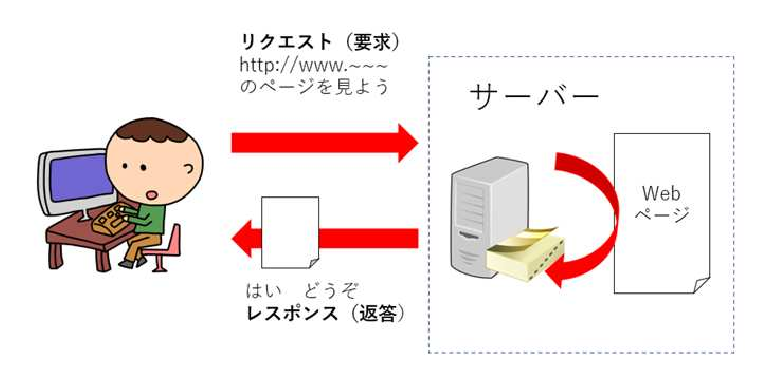
\includegraphics[width=0.75\textwidth]{ome7-img049}
\flushleft


webブラウザで検索したりしてwebページを表示させることをリクエスト(要求)といい、そのリクエストを受け取ったそのwebページのあるサーバーが要求したところにレスポンス(返答)を返します。要求されたら返すのみで、webページに変化はなく同じものを見せていました。ですが次の画像をみてください。


\bigskip

\centering
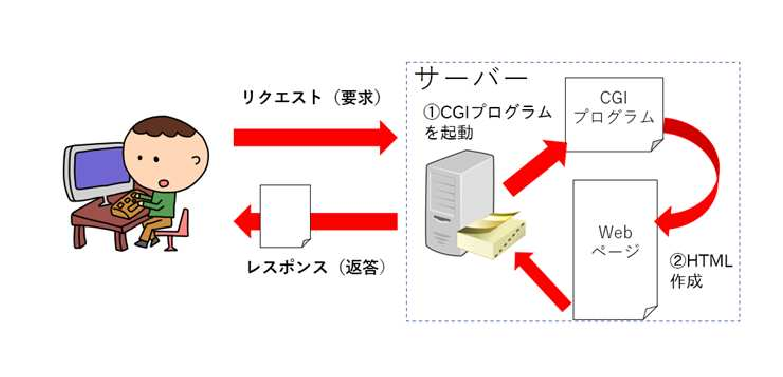
\includegraphics[width=0.75\textwidth]{ome7-img050}
\flushleft


CGIを使った動的ページでは、サーバーが皆さんからwebページを要求されるたびに、CGIプログラムで新しいHTMLを生成しています。それにより、毎回違うwebページを見せることが可能なのです。この教科書では皆さんのラズベリーパイと今までの講義で学んだことを生かしたCGIを体験していきます。


\bigskip

\refstepcounter{Question}\theQuestion 動的なページとはどのようなものでしょうか。また、動的なページを作成する場合に用いるものは何でしょう。\label{Q:dynamicPage}



\addBlank{答え}


\addBlank{答え}


\refstepcounter{Exercise}
\clearpage\subsection*{\theExercise CGIを使ってウェブページからLEDをつける}
\addtocounter{Exercise}{-1}\refstepcounter{Exercise}\label{E:CGI}
考え方

まずはラズパイにセンサーボードを取り付けましょう。今回はFaBoは使用しません。

ウェブサーバはウェブブラウザから要求を受けます。”ファイル名.hsp”ファイルへのアクセスをブラウザから行うとサーバはCGIプログラムをサーバ側で起動します。結果はHTMLとしてブラウザ(クライアント)へ返されます。

試しに、CGIプログラムを起動させてみましょう。例題のプログラムはLEDがすでに点灯していれば消灯、消灯してれば点灯するプログラムです。ウェブサーバがウェブブラウザから要求を受けて、CGIプログラムを起動するのでウェブサーバが起動している必要があります。まずはウェブサーバを起動させましょう。

ターミナルを開いて

cd {\textasciitilde}/07/www/

./webserver.py \ \ \ \ で起動できます。

%
%コマンド実行画面
%cd {\textasciitilde}/07/www/
%./webserver.py
%koyaman
%September 20, 2019 2:48 AM


次にウェブブラウザからウェブサーバへCGIの要求を出してみましょう。

ブラウザを開いて、

localhost:3000/cgi-bin/led.hsp

%
%ぶらうざで開いた画面
%koyaman
%September 20, 2019 2:49 AM


\centering
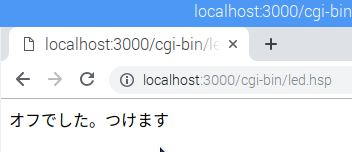
\includegraphics[width=0.7\textwidth]{ome7-img051.png}
\flushleft

にアクセスをしてみましょう。アクセスをすると、プログラムが起動してLEDが点灯します。ブラウザのリロードボタンを押すと消灯します。

\centering
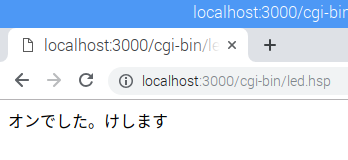
\includegraphics[width=0.7\textwidth]{ome7-img052.png}
\flushleft

cgi-binディレクトリはCGIプログラムを入れるディレクトリです。{\textasciitilde}/07/wwwの下にあります。このディレクトリ内の

”ファイル名”.hsp

はCGIプログラムとして\ruby{扱}{あつ}われます。led.hspはCGIプログラムです。


\bigskip

\clearpage
プログラム解説



\centering
\begin{boxedminipage}{0.95\textwidth}

	\begin{enumerate}
	\baselineskip 10pt
	\setlength{\itemsep}{0cm}
	\item \#include {\textquotedbl}hsp3cl.as{\textquotedbl}

	\item \#include {\textquotedbl}rpz-gpio-cl.as{\textquotedbl}


	\item

	\item mes {\textquotedbl}Content-type: text/html{\textbackslash}n{\textquotedbl}

	\item mes {\textquotedbl}{\textless}html{\textgreater}{\textless}head{\textgreater}{\textless}meta
	charset={\textbackslash}{\textquotedbl}utf-8{\textbackslash}{\textquotedbl}{\textgreater}{\textless}/head{\textgreater}{\textless}body{\textgreater}{\textquotedbl}


	\item

	\item ;現在のGPIO 17の\ruby{値}{あたい}を取得 1 == ON, 0 == OFF

	\item ;CGIからはcgpioinを使う(使い方はgpioinと同じ)

	\item prev\_led = cgpioin(17)

	\item

	\item if prev\_led = 0\{

	\item ;ついていなかった

	\item mes
		{\textquotedbl}{\textless}p{\textgreater}オフでした。つけます{\textless}/p{\textgreater}{\textquotedbl}

	\item next\_led = 1

	\item \}else\{

	\item ;

	\item mes
		{\textquotedbl}{\textless}p{\textgreater}オンでした。けします{\textless}/p{\textgreater}{\textquotedbl}

	\item next\_led = 0

	\item \}

	\item mes {\textquotedbl}{\textless}/body{\textgreater}{\textless}/html{\textgreater}{\textquotedbl}

	\item ;CGIからはcgpioを使う(使い方はgpioと同じ、0以外を書いた場合プログラムが

	\item ;\ruby{終了}{しゅうりょう}してもLEDは点灯し続ける)

	\item cgpio 17, next\_led

	\item end
	\end{enumerate}

\end{boxedminipage}
\flushleft



第3回に使用した命令ではない命令が入っています。\\
詳細はP\pageref{P:gpio}に載っています。確認してください。

プログラム解説の4行目

mes {\textquotedbl}Content-type: text/html{\textbackslash}n{\textquotedbl}

はCGIプログラムがウェブサーバに結果を返すときに、結果がHTMLであることを伝えるために必要です。{\textbackslash}nは改行を意味します。本来は改行は2つ必要ですが、mes命令は自動で改行を入れてくれるので、{\textbackslash}nは1つで十分です。


\bigskip
\clearpage
4行目\ruby{以降}{いこう}のmes命令で出力するものは、HTMLの一部として扱われます。

\bigskip

6行目では、文字コードを設定しています。

\bigskip

9行目からLED点灯消灯のプログラムが始まります。

prev\_led = cgpioin(17)

では、GPIO17番の状態を調べています。LEDが点灯していれば1になり、消灯していれば0になります。


\bigskip


10〜17行目では、\ruby{条件}{じょうけん}判断のif文を使って読み取ったLEDの状態を判断します。消灯状態であれば、9行目で

mes
	{\textquotedbl}{\textless}p{\textgreater}オフでした。つけます{\textless}/p{\textgreater}{\textquotedbl}

pタグを使ってメッセージを表示します。

\bigskip

12行目で

next\_led = 1

としてLEDを点灯させるための値を用意します。

\bigskip

消灯以外の状態(つまり点灯状態)の場合は、13行目で

mes
	{\textquotedbl}{\textless}p{\textgreater}オンでした。けします{\textless}/p{\textgreater}{\textquotedbl}

pタグを使ってメッセージを表示します。

\bigskip

18行目で

next\_led = 0

としてLEDを消灯させるための値を用意します

\bigskip

20行目で実際に値をGPIO17へ書き込みます。

cgpio 17, next\_led




\bigskip

21行目の

end

でプログラムの終了をします。


\bigskip



第7回のCGIを使うプログラムでは、第3回の授業とはちがう命令を使います。\\
第3回の命令でCGIを使おうとすると、上手く動かなくなってしまうからです。\\
下の表にそれぞれの命令をまとめておきます。\\

\clearpage
\refstepcounter{PagePtr}\label{P:gpio}
\begin{flushleft}
	\tablefirsthead{}
	\tablehead{}
	\tabletail{}
	\tablelasttail{}
	\begin{supertabular}{|m{5.0cm}|m{5.5cm}|m{7.0cm}|}
		\hline
		第3回に使った
		命令名 &
		CGIを使うときの
		命令名&
		効果
		\\\hline

		\#include “rpz-gpio.as”&
		\#include “rpz-gpio-cl.as”&
		プログラムのはじめに書くことでLED
		の点灯や消灯の命令が使えるようになります。
		\\\hline

		onoff\ = \ gpioin(17)&

		onoff\ = \ cgpioin(17)&
		17番のGPIOのLEDが点灯していれば変数onoffに1が、
		消灯していれば変数onoffに0が入ります。
		17をほかの番号に変えることで、
		ほかのLEDの状態を確認できます。
		\\\hline

		gpio \ 18,\ 1&
		cgpioin \ 18,\ 1&
		18番のGPIOのLEDを点灯します。
		1を0にすると消灯になります。
		18をほかの番号に変えることで、
		ほかのLEDを点灯、消灯できます。
		\\\hline



	\end{supertabular}
\end{flushleft}






\bigskip


\bigskip
\refstepcounter{Question}\theQuestion

{\bfseries
	友達のLEDをCGIで点灯させてみよう。}

{\bfseries

	点灯、消灯時のウェブページに表示されるメッセージを\ruby{変更}{へんこう}してみよう。}

{\bfseries
	他の色のLEDも点灯、消灯できるようにしよう。}

{\bfseries
	Faboのセンサ(LED,
	\ruby{振動子}{しんどうし}などのデジタルセンサ)を接続してCGIから動かせるようにしてみよう。}


\bigskip

\refstepcounter{Exercise}
\clearpage\subsection*{\theExercise URLを使ってCGIに情報を\ruby{渡}{わた}す}
\addtocounter{Exercise}{-1}\refstepcounter{Exercise}\label{E:URL}
考え方

CGIのプログラムに情報を渡すことができればより便利なプログラムが作れます。ここでは\ruby{単純}{たんじゅん}なURLを用いた方法を使います。URLに\ruby{埋}{う}め込まれた情報はクエリストリングと呼ばれます。クエリストリングはまずウェブサーバへ送られ、ウェブサーバがCGIプログラムへクエリストリングを渡します。これによりCGIプログラムはURLに埋め込まれた情報を扱うことができます。


\bigskip

まずは、ブラウザを開いて、

localhost:3000/cgi-bin/querystring.hsp?msg=helloworld

を入力してみましょう。

%
%ぶらうざで開いた画面
%helloworldと表示されている
%koyaman
%September 20, 2019 2:49 AM


画面にhelloworldと表示されたと思います。



\centering
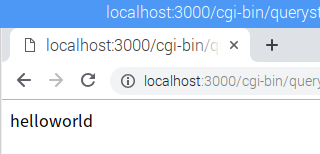
\includegraphics[width=0.8\textwidth]{ome7-img053.png}
\flushleft

localhost:3000/cgi-bin/querystring.hsp?msg=goodbye

に変更してみてください。

%
%ぶらうざで開いた画面
%goodbyeと表示されている
%koyaman
%September 20, 2019 2:49 AM


次はgoodbyeと表示されたと思います。


\centering
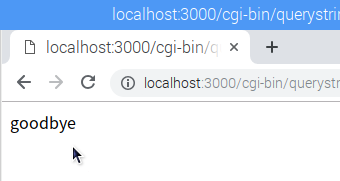
\includegraphics[width=0.8\textwidth]{ome7-img054.png}
\flushleft

\clearpage

このようにURLに情報を埋め込んでおくことでCGIのプログラムはこれを受け取り処理をすることができます。URLに埋め込まれた情報はクエリストリングと呼ばれます。この情報はまずウェブサーバが受け取ります。ウェブサーバは少し\ruby{処理}{しょり}をしてCGIプログラムへ渡します。

クエリストリングはURLの最後に?をつけて始めます。

クエリストリングの形は

名前=値

のようになっています。この例では

msg=helloworld

msg=goodbye

などとなっています。これはmsgという名前の値はhelloworld,
goodbyeであることを意味します。HSPの変数と同じような感じです。

次にCGIプログラムでどのようにクエリストリングを扱っているのか見てみましょう。


\bigskip

プログラム解説



\centering
\begin{boxedminipage}{16.233cm}
	\begin{enumerate}
	\baselineskip 10pt
	\setlength{\itemsep}{0cm}
	\item\#include {\textquotedbl}hsp3cl.as{\textquotedbl}

	\item\#include {\textquotedbl}cgi.as{\textquotedbl}

	\item mes {\textquotedbl}Content-type: text/html{\textbackslash}n{\textquotedbl}

	\item mes {\textquotedbl}{\textless}html{\textgreater}{\textless}head{\textgreater}{\textless}meta
		charset={\textbackslash}{\textquotedbl}utf-8{\textbackslash}{\textquotedbl}{\textgreater}{\textless}/head{\textgreater}{\textless}body{\textgreater}{\textquotedbl}

	\item getqueryval {\textquotedbl}msg{\textquotedbl}, q

	\item mes q

	\item mes {\textquotedbl}{\textless}/body{\textgreater}{\textless}/html{\textgreater}{\textquotedbl}

	\item end
	\end{enumerate}
\end{boxedminipage}
\flushleft


\bigskip


\bigskip

5行目の

getqueryval “msg”, q

はクエリストリング内の名前が”msg”に対応する値を変数qに入れています。

localhost:3000/cgi-bin/querystring.hsp?msg=helloworld

というURLがあった場合、

変数qにはhelloworldが文字列として入ります。

6行目で表示をしています。

このように\ruby{簡単}{かんたん}にプログラムでクエリストリングを受け取ることができます。クエリストリングが使えると、{\textless}form{\textgreater}{\textless}/form{\textgreater}を使ってCGIに処理を\ruby{依頼}{いらい}できたり、CGIの処理をより高度にすることができます。次の例では、クエリストリングを使ってLEDを点灯消灯します。

ほとんどのウェブサイトは検索をするさいにURLに検索ワードを埋め込んでいます。


\bigskip

\refstepcounter{Question}\theQuestion 画面に”ありがとう”と表示させよう。

	\refstepcounter{Exercise}
\clearpage\subsection*{\theExercise クエリストリングを使ってLEDを操作する}
\addtocounter{Exercise}{-1}\refstepcounter{Exercise}\label{E:QS}
この例では、クエリストリングを使ってLEDを点灯消灯させてみましょう。


\bigskip

まずは、ブラウザを開いて、

localhost:3000/cgi-bin/qsled.hsp?led=17\&val=1

を入力してみましょう。

%
%ぶらうざで開いた開いた画面
%koyaman
%September 20, 2019 2:50 AM


\centering
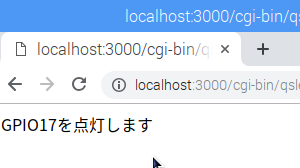
\includegraphics[width=0.8\textwidth]{ome7-img055.png}
\flushleft

実行するとLED17が光ります。val=1をval=0にすると消えます。URLに埋め込まれた情報をもとにCGIプログラムはLEDを操作していることがわかります。URLに埋め込まれた情報はクエリストリングと呼ばれます。


\bigskip

クエリストリングを\ruby{詳}{くわ}しく見てみましょう。

クエリストリングとはURLの最後に?をつけて始めます。?のあとには

名前(変数名みたいなもの) = 値

の形を続けます。例えば、

localhost:3000/cgi-bin/qsled.hsp?led=17

のようにかけます。この場合は、

名前がled、値が17となります。

複数の情報を渡したい場合は\&を使います。

localhost:3000/cgi-bin/qsled.hsp?led=17\&val=1

のようになります。

名前1がled、値1が17となり

名前2がval、値2が1となります。

このクエリストリングをプログラムから扱う方法を次に学びましょう。

\clearpage
プログラム解説



\centering
\begin{boxedminipage}{16.538cm}
	\begin{enumerate}
	\baselineskip 10pt
	\setlength{\itemsep}{0cm}
	\item\#include {\textquotedbl}hsp3cl.as{\textquotedbl}

	\item\#include {\textquotedbl}rpz-gpio-cl.as{\textquotedbl}

	\item\#include {\textquotedbl}cgi.as{\textquotedbl}

	\item mes {\textquotedbl}Content-type: text/html{\textbackslash}n{\textquotedbl}

	\item mes {\textquotedbl}{\textless}html{\textgreater}{\textless}head{\textgreater}{\textless}meta
		charset={\textbackslash}{\textquotedbl}utf-8{\textbackslash}{\textquotedbl}{\textgreater}{\textless}/head{\textgreater}{\textless}body{\textgreater}{\textquotedbl}

	\item; クエリストリングからledを探して、値をled\_portへ入れる

	\item getqueryval {\textquotedbl}led{\textquotedbl}, led\_port

	\item ; クエリストリングからvalを探して、値をled\_valへ入れる

	\item getqueryval {\textquotedbl}val{\textquotedbl}, led\_val

	\item ;文字列なので数値へ変換する

	\item led\_port = int(led\_port)

	\item led\_val = int(led\_val)


	\item

	\item; 点灯消灯を判断して、メッセージをpタグで表示する

	\item if(led\_val = 1) \{

	\item\ \ \ \ mes {\textquotedbl}{\textless}p{\textgreater}GPIO{\textquotedbl} + led\_port +
		{\textquotedbl}を点灯します{\textless}/p{\textgreater}{\textquotedbl}

	\item\} else \{

	\item\ \ \ \ mes {\textquotedbl}{\textless}p{\textgreater}GPIO{\textquotedbl} + led\_port +
		{\textquotedbl}を消灯します{\textless}/p{\textgreater}{\textquotedbl}

	\item\}


	\item

	\item;クエリストリングのledで指定されたGPIOにvalで指定された値を書き込む

	\item; localhost:3000/cgi-bin/qsled.hsp?led=17\&val=1

	\item; の場合、LED17を点灯させる

	\item cgpio led\_port, led\_val

	\item mes {\textquotedbl}{\textless}/body{\textgreater}{\textless}/html{\textgreater}{\textquotedbl}

	\item end
	\end{enumerate}
\end{boxedminipage}
\flushleft

\bigskip



\bigskip


\bigskip

7行目、9行目で使用している

getqueryval命令でクエリストリングを受け取ります。この命令は

getqueryval 名前, 値を入れる変数

のように使います。クエリストリングから名前を探して、変数へ値を文字列としていれます。

例えば、

getqueryval led, led\_port

の場合にlocalhost:3000/cgi-bin/qsled.hsp?led=17

とクエリストリングを与えたとすると、

led\_portには17が入ります。

11,12行目で

文字列から数値へ変換しています。

15〜19行目では、点灯するのか消灯するのかを条件判断を使って判断しています。led\_valが1のとき(val=1がクエリストリングで与えられたとき)に点灯する、その他のときは消灯するとします。

24行目で実際に点灯、消灯を行います。

cgpio命令は数値でGPIO番号、オンオフ(1,0)を受け付けるので、文字列から変換をしました。


\bigskip

\refstepcounter{Question}\theQuestion

{\bfseries
	GPIO17以外のLEDを光らせてみよう。}


\bigskip


\bigskip
